\chapter{Metodologia} \label{metodologia}

Este trabalho utilizou uma metodologia .

\section{Definição do Componente}

Dentro do campo de içamento 

\begin{figure}[!htb]
   \centering
     \caption{Componentes da manilha.}
    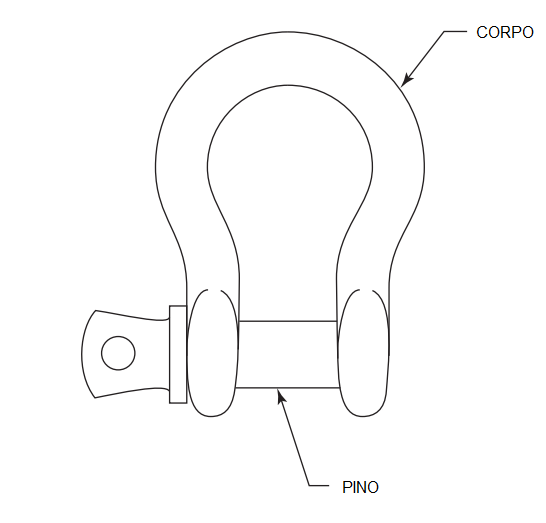
\includegraphics[width=0.45\linewidth]{Figuras/manilhacomponentes.png}\\
    \hspace{1.5cm}\raggedright \fontsize{10}{12}\selectfont{Fonte: Adaptado de \textcite{ASMEB3026}.}
    \label{manilhacomponentes}
\end{figure}

Manilhas comerciais possuem um formato típico, basicamente composto por um corpo em formato de arco e um pino de travamento, conforme  \ref{manilhacomponentes}. Existem muitas combinações possíveis para a montagem de manilhas em um conjunto de içamento e movimentação, entre essas combinações estão as montagens que se utilizam de múltiplas manilhas acopladas, como exemplificado na  \ref{manilhacombinacoes}. Visando essas combinações, a proposta deste trabalho é reproduzir essa combinação corpo-corpo em uma geometria única, de modo a verificar seu comportamento diante das solicitações de trabalho esperadas para o componente.

\begin{figure}[!htb]
   \centering
     \caption{Combinações de manilhas.}
    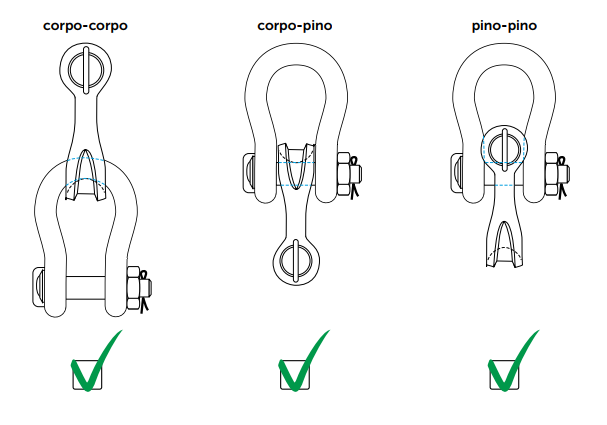
\includegraphics[width=0.65\linewidth]{Figuras/manilhacombinacoes.png}\\
    \hspace{1.5cm}\raggedright \fontsize{10}{12}\selectfont{Fonte: \textcite{GreenPin}.}
    \label{manilhacombinacoes}
\end{figure}

Como referência, foi utilizado a Super\textsuperscript{\textregistered}\hspace{0.1em} Manilha Curva SC, da Green Pin\textsuperscript{\textregistered}\hspace{0.1em}, padrão de excelência na fabricação e comercialização de manilhas no mercado internacional, conforme anexo A. Com corpo e pino em aço liga, grau 8, temperado e revenido.

Para requisitos iniciais, foram estabelecidos os parâmetros para verificação da geometria inicial conforme a  \ref{parametrosinicicais}. Como material do componente, foi escolhido o aço AISI 4340, com as propriedades mecânicas do componente tratado termicamente por têmpera e revenimento.

\begin{table}[!ht]
\centering
\caption{Parâmetros iniciais.}
\label{parametrosinicicais}
\begin{tabular}{ P{3cm} | P{3cm} | P{3cm} | P{3cm} } 
\hline
\textbf{Carregamento de Trabalho (kN)} & \textbf{Massa do Componente (kg) } & \textbf{Fator de segurança - FS} & \textbf{Diâmetro do Pino (mm)} \\ \hline
 10 & 1,0 & 5:1 & 19 \\ 
\hline
\end{tabular} \\
\smallskip
\hspace{1.5cm}\raggedright \fontsize{10}{12}\selectfont{Fonte: Elaborado pelo autor, 2025.}
\end{table}
